\documentclass[12pt, titlepage]{article}

\usepackage{amsmath, amssymb}
\usepackage[margin=0.75in]{geometry}

\usepackage{graphicx}
\graphicspath{{./img/}}

\usepackage{listings}
\usepackage{color}
\definecolor{mygreen}{rgb}{0,0.6,0}
\definecolor{mygray}{rgb}{0.5,0.5,0.5}
\definecolor{mymauve}{rgb}{0.58,0,0.82}

\lstset{ 
  backgroundcolor=\color{white},
  basicstyle=\footnotesize\ttfamily,
  breakatwhitespace=false,
  breaklines=true,
  captionpos=b,
  commentstyle=\color{blue},
  extendedchars=true,
  frame=tb,
  keepspaces=true,
  keywordstyle=\color{mymauve},
  numbers=left,
  numberstyle=\footnotesize\ttfamily\color{mygray},
  rulecolor=\color{black},
  showspaces=false,
  showstringspaces=false,
  showtabs=false,
  stepnumber=1,
  stringstyle=\color{mygreen},
  morestring=[d]",
  tabsize=2,
  title=\lstname
}

\lstdefinestyle{cypher}{
  morekeywords={CREATE, MATCH, WHERE, RETURN, AND, IN},
}

\lstdefinestyle{mql}{
  morekeywords={
    WHO,
    WHEN,
    WHAT,
    WHERE,
    DESCRIPTION,
    head,
    parent,
    branchName,
    active,
    timestamp,
    created
  }
}

\renewcommand{\refname}{Références}

\title{\textbf{IFT4055 - Projet Honor} \\ MQL à Cypher -- Un Framework pour
  Traduire un langage de requêtes spécifique au domaine pour interroger un
  projet versionnable en des expressions Cypher}
\author{Philippe Gabriel - 20120600}
\date{18 décembre 2022}

\begin{document}

\maketitle
\pagenumbering{arabic}
\setcounter{page}{2}

\section*{Problème}

Les systèmes de versions de contrôle (\textit{Version Control System} -- VCS)
présentent une grande importance dans les besoins de vouloir gérer le
versionnement de collections de données. Dans le domaine de l'informatique et de
l'ingénierie logicielle, des systèmes comme Git représentent une très grande
importance dans la pratique menant à l'intérêt industrielle du développement de
grands logiciels. L'ingénierie dirigée par les modèles (\textit{Model-Driven
Engineering} -- MDE) est une approche présentant plusieurs avantages dans la
conception de logiciels. Cette approche permet au concepteur d'abstraire des
détails des langages de programmation générals, de sorte à concentrer ses
efforts dans la résolution du problème. L'usage de modèles ou de langages
spécifiques au domaine (\textit{Domain-Specific Languages} -- DSL) aide l'expert
à s'exprimer dans une terminologie propre à son domaine d'étude et lui
permettrait de contribuer à la conception d'un logiciel sans avoir de
connaissances de programmation. Un intérêt industrielle commence à se manifester
pour la MDE poussant à l'adopter pour concevoir de larges projets. Un VCS
orienté-ligne comme Git utilisé pour gérer le versionnement des changements
apporter à un projet MDE n'est pas la meilleure approche à adopter gérer de gros
projets. L'interprétation des changements sur un modèle conçu par l'expert du
domaine sera au niveau de la sérialisation du modèle. Cette interprétation n'est
donc pas spécifique au domaine du modèle. La sémantique riche du domaine est
complètement négligé. Un VCS spécifique au domaine (\textit{Domain-Specific VCS}
-- DSVCS) serait plus approprié pour des projets MDE. DSMCompare
\cite{dsmcompare} permet de comprendre les différences entre modèles en terme de
la sémantique d'un langage de modélisation. Il s'agit d'une approche considérant
la syntaxe abstraite et concrète d'une DSL pour exprimer les différences entre
modèles. Ce niveau de détection de changements est une composante cruciale dans
un DSVCS. Un DSVCS devrait adhérer à différents critères tel que la définition
d'une unité versionnable pour permettre la comparaison sémantique, les commandes
offertes pour manipuler le projet, la possibilité d'interroger le VCS selon le
projet, la méthode de stockage, etc... \cite{dsvcs}. Pour ce projet, je présente
une approche MDE basé sur la traduction d'expressions MQL -- un langage de
requêtes spécifique au domain (\textit{Domain-Specific Query Language} -- DSQL)
pour interroger un projet versionnable -- en des expressions Cypher -- un
langage de requêtes supporté par des bases de données de graphes Neo4j. Ce
projet vient essentiellement proposer une solution quant à la composante
d'interroger le VCS.

\section*{Méthodes utilisées}

La solution proposée est basée sur la MDE. Sa presque totalité a donc été
rédigée dans le Eclipse Modeling Framework (EMF). Je présente, dans les
sous-sections ci-dessus, les différentes étapes de la solution.

\subsection*{Projet Versionnable}

\begin{figure*}
  \centering
  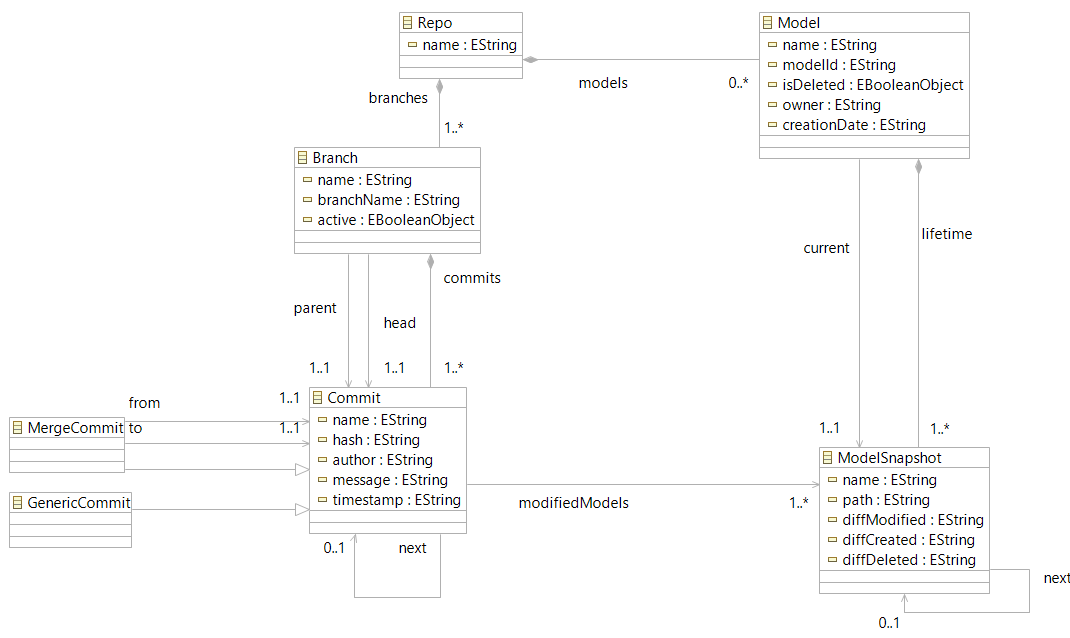
\includegraphics[width=\textwidth]{repomm.png}
  \caption{Métamodèle d'un Projet Versionnable}
  \label{fig:repomm}
\end{figure*}

Afin d'interroger le VCS sur un projet versionnable, il est nécessaire de
déterminer à priori les unités versionnables d'un projet. Cela est décrit dans
le métamodèle d'un projet versionnable présenté à la Figure \ref{fig:repomm}. Un
projet versionnable a une structure assez similaire à celle des projets
utilisant un VCS linéaire. Un projet consiste en des branches. Les branches
contiennent des commits définissant un point où l'on désire enregistrer des
changements. Les modèles constituent ici l'unité dont l'expert du domaine
modifiera dans le projet MDE. Chaque modèle possède une durée de vie exprimée
sous forme d'une série de snapshots.

\subsection*{Model Query Language - MQL}

\begin{figure}[ht!]
  \centering
  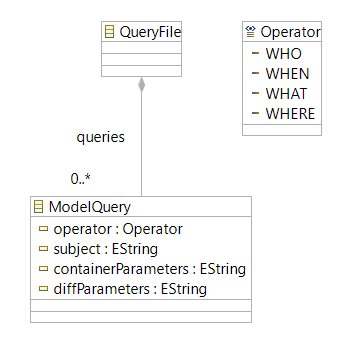
\includegraphics[width=0.4\textwidth]{mqlmm.png}
  \caption{Métamodèle de MQL}
  \label{fig:mqlmm}
\end{figure}

La syntaxe abstraite du langage MQL est exprimé dans le métamodèle de MQL à la
Figure \ref{fig:mqlmm}. Une expression MQL est constituée de plusieurs requêtes.
Chaque requête est composée d'un opérateur, du sujet de requête, et de
paramètres pour mieux filtrer les résultats attendues. La syntaxe concrète de ce
langage a été définie à l'aide de Xtext. Le Listing \ref{lst:mqlsyn} démontre un
exemple d'expression MQL. Dans cette expression, on remarque que chaque requête
est séparée par une virgule et que la dernière requête se termine par un point
d'interrogation. Chaque requête commence par un opérateur. La seconde requête
utilise l'opérateur \texttt{DESCRIPTION} qui s'agit ici tout simplement de sucre
syntaxique pour l'opérateur \texttt{WHERE} qui a été jugé ne pas être très
intuitif dans ce contexte.

\begin{lstlisting}[style=mql, label=lst:mqlsyn, caption=Expression MQL]
  WHO head {
    branchName = "main",
    active = "true"
  },
  DESCRIPTION parent {
    branchName = "b1"
  },
  WHEN created {
    timestamp < "2022-09-04"
  } [
    "MyDomainSpecificObject.x = 19"
  ]?
\end{lstlisting}

Un parseur Xtend a été implémenté pour produire un modèle MQL à partir d'une
expression MQL. Ce dernier génère un modèle MQL conforme au métamodèle MQL
lorsque l'expert du domaine sauvegarde le fichier où il rédigeait ses requêtes
MQL.

\subsection*{Transformations Modèle-à-texte}

À partir d'un modèle d'un projet versionnable conforme à son métamodèle.

\subsection*{Automatisation}

\section*{Résultats obtenus}

\section*{Améliorations futures}

\bibliographystyle{plain} 
\bibliography{refs}

\end{document}

